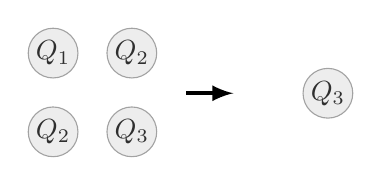
\begin{tikzpicture}[>=latex]
\def\Length{1}
\def\Radius{0.07}

% pre coarsening
\LagrangeCell{0}{0}{\Length}{\Radius}{2}
  {{,,,,,,,,}};
\node[circle, draw=gray, fill=gray!20, inner sep=1pt, opacity=0.7, text opacity=0.8] at (0.5\Length,0.5\Length) {$Q_2$};

\LagrangeCell{\Length}{0}{\Length}{\Radius}{3}
  {{,,,,,,,,,,,,,,,}};
\node[circle, draw=gray, fill=gray!20, inner sep=1pt, opacity=0.7, text opacity=0.8] at (1.5\Length,0.5\Length) {$Q_3$};

\LagrangeCell{0}{\Length}{\Length}{\Radius}{1}
  {{,,,}};
\node[circle, draw=gray, fill=gray!20, inner sep=1pt, opacity=0.7, text opacity=0.8] at (0.5\Length,1.5\Length) {$Q_1$};

\LagrangeCell{\Length}{\Length}{\Length}{\Radius}{2}
  {{,,,,,,,,}};
\node[circle, draw=gray, fill=gray!20, inner sep=1pt, opacity=0.7, text opacity=0.8] at (1.5\Length,1.5\Length) {$Q_2$};

% arrow
\draw[->,ultra thick] (2.2*\Length,\Length) -- (2.8*\Length,\Length);

% post coarsening
\LagrangeCell{3*\Length}{0}{2*\Length}{\Radius}{3}
  {{,,,,,,,,,,,,,,,}};
\node[circle, draw=gray, fill=gray!20, inner sep=1pt, opacity=0.7, text opacity=0.8] at (4*\Length,\Length) {$Q_3$};
\end{tikzpicture}